\documentclass[a4paper, 12pt]{report}
\usepackage[utf8]{inputenc} 
\usepackage[T1]{fontenc}
\usepackage[frenchb]{babel} %ou \usepackage[francais]{babel} 
\usepackage{url} %écrire des adresses cliquables
\usepackage{lmodern} %changer pack de police
\usepackage[top=3cm, bottom=3cm, left=2.5cm, right=2.5cm]{geometry} %gérer les marges
\usepackage{color}
\usepackage[babel=true]{csquotes} % csquotes va utiliser la langue définie dans babel
\usepackage{graphicx}
\usepackage[space]{grffile}
\usepackage{listings}
\lstset{language=C,basicstyle=\small,frame=leftline,captionpos=b,linewidth=175mm,breaklines=true, ,identifierstyle=\ttfamily, numbers=none, numberstyle=\tiny, stepnumber=5, numberfirstline=true, showstringspaces=false}
\input{milstd}
\DeclareGraphicsExtensions{.jpeg, .png , .gif, .bmp}
\usepackage{eurosym}
\usepackage{array}
\newcolumntype{M}[1]{>{\raggedright}m{#1}}
\usepackage{wrapfig}


%%%%%%%%%%%%%%%%%%%%%%%%%
\begin{document}


% placement des elements
\makeatletter
	\def\clap#1{\hbox to 0pt{\hss #1\hss}}%
	\def\ligne#1{%
	\hbox to \hsize{%
	\vbox{\centering #1}}}%
	\def\haut#1#2#3{%
	\hbox to \hsize{%
	\rlap{\vtop{\raggedright #1}}%
	\hss
	\clap{\vtop{\centering #2}}%
	\hss
	\llap{\vtop{\raggedleft #3}}}}%
	\def\bas#1#2#3{%
	\hbox to \hsize{%
	\rlap{\vbox{\raggedright #1}}%
	\hss
	\clap{\vbox{\centering #2}}%
	\hss
	\llap{\vbox{\raggedleft #3}}}}%
	\def\maketitle{%
	\thispagestyle{empty}\vbox to \vsize{%
	\haut{}{\@blurb}{}
	\vfill
	\vspace{1cm}
\begin{flushleft}
	\usefont{OT1}{ptm}{m}{n}
	\huge \@title
\end{flushleft}
	\par
	\hrule height 4pt
	\par
\begin{flushright}
	\usefont{OT1}{phv}{m}{n}
	\Large \@author
	\par
\end{flushright}
	\vspace{1cm}
	\vfill
	\vfill

\begin{center}
	
\includegraphics[width=7cm]{logo_UTBM2.jpg}
\end{center}

\bas{}{Printemps 2013}{}
}%
\cleardoublepage
}
\def\date#1{\def\@date{#1}}
\def\author#1{\def\@author{#1}}
\def\title#1{\def\@title{#1}}
\def\location#1{\def\@location{#1}}
\def\blurb#1{\def\@blurb{#1}}
\date{\today}
\author{}
\title{}

% informations
\location{Belfort}\blurb{}
\makeatother
\title{Rapport de projet - Affectation des fréquences dans les réseaux mobiles}
\author{\small{Thomas Gloriod, Paul Locatelli et Pierre Rognon}}
\blurb{%
	\textbf{AG41 - Optimisation et recherche opérationnelle}\\
	Université de Technologie de Belfort-Montbéliard
}% 


\maketitle
\tableofcontents 
%%%%%%%%

\chapter{Présentation du sujet}
Le problème d'affectation de fréquences est un problème type en recherche opérationnelle. Ce problème s'apparente à un problème de coloration de graph.
Il s'agit ici d'attribuer des fréquences à différents secteurs d'une même zones. Deux secteurs limitrophes ne pouvant pas émettre sur la même fréquence.

\section{Détails du problème}
Le département étudié, ici le Territoire de Belfort comporte 36, chacun étant divisé en maximum trois secteurs pour un total de 88 secteurs. Chaque secteur d'un même site émet sur la sous-bande fréquence 1, 2 ou 3. 

\begin{center}
	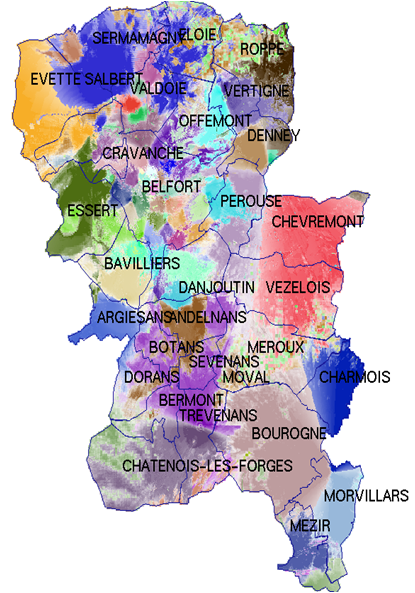
\includegraphics[scale=1]{carte.png} 
	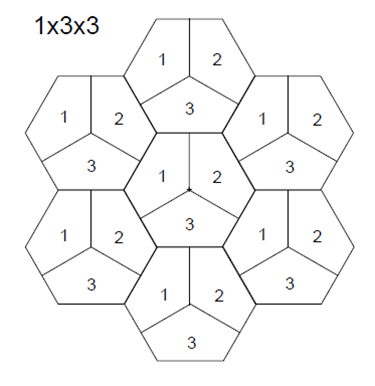
\includegraphics[scale=1]{ruche.png} 
\end{center}

Pour que les clients soient couvert, les secteurs ayant une frontière communes doivent avoir des fréquences différentes afin de minimiser les interférences. Au sein du territoire 12 695 points test permettent d'évaluer la qualité de l'allocation des fréquences. Chaque points test est caractérisé par un nombre de clients et le débit qu'il souhaite avoir. Le nombre de clients n'ayant pas accès au réseau est donc la fitness à minimiser.

\section{Objectifs}
Afin d'assurer l'accès au réseau au maximum de clients, il s'agit d'allouer les fréquences à chaque secteur de chaque sites de manière à minimiser le nombre de clients non-couvert par le réseau.

\chapter{Principe de résolution}
Pour résoudre ce type de problème, l'utilisation de méthode exacte demanderait le calcul de 6\up{36} soit environ 10\up{28} allocation de fréquences différentes. C'est pourquoi pour ce genre de problème ou le nombre de solution est trop importante, les méthode de résolution approchée sont utilisées.

\section{Méthode approchées}
Le principe de cette méthode de résolution est simple. On cherche d'abord une solution au problème, soit de manière aléatoire, soit en en calculant pas trop mauvaise.
On définit ensuite une liste de voisin à cette solution. Un voisin d'une solution suit des règles précises, définit au préalable. On calcule la fitness de tous les voisins et on garde la meilleur solution trouvées parmi elles. Il suffit ensuite de réitérer l'opération sur la nouvelle solution afin d'améliorer le résultat jusqu'à ce qu'aucun voisin ne soit meilleur que la solution courante.

\section{La recherche tabou}
La recherche tabou est une amélioration de l'algorithme énoncé précédemment. Le principe est similaire cependant lorsqu'une solution voisine est étudiée, elle est placé ensuite dans la liste tabou pendant plusieurs itérations et ne pas reconsidérée. Cet optimisation permet de ne pas perdre de temps en recalculant les mêmes solutions à chaque fois.

\chapter{Algorithme développé}
\section{Génération de la solution initiale}
\section{Implémentation de la recherche tabou}

\chapter{Résultats observés}

\chapter{Conclusion}
L'algorithme de recherche tabou est fonctionnel. Il permet d'obtenir une fitness très satisfaisante afin d'offrir aux clients la meilleur couverture réseau.

Des améliorations restent possibles en modifiant la méthode du choix des voisins à chaque itération, ou en modifiant la durée de la liste tabou.\\

L'exercice est intéressant car il demande de s'immiscer dans un programme déjà existant, de le comprendre afin d'y ajouter les fonctions à développer. C'est un exercice réaliste puisque dans le monde de l'entreprise, les programmes à développer partent rarement de zéro.\\

Ce projet nous a également permis de nous perfectionner dans le langage C++, de découvrir de nouvelles subtilités et d'améliorer notre manière de programmer. Pour partager les sources du programme, l'utilisation d'un logiciel de gestion de version facilite la tâche.\\

Enfin ce projet a été une expérience enrichissante car effectué au sein d'un groupe de trois étudiants. La communication est importante ainsi que la répartition des tâches. Le travail en groupe permet le partage des compétences et des idées. \\

\appendix
\chapter{Génération de la solution initiale}
\begin{lstlisting}
int* site::randomizeTableFreq(){
    int* tableFreq = new int[3];
    int* table = new int[3]; for(int i=0; i<3;i++)table[i]=i+1;
    int* tableTmp = NULL;
    int taille = 3;
    long random;
    bool shift;
    for(int i=0; i<3; i++)
    {
        shift = false;
        random = Random::aleatoire(taille);
        tableFreq[i]=table[random];
        tableTmp = new int[taille-1];
        for(int j=0; j<taille; j++)
        {
            if(j != random){
                if(shift) tableTmp[j-1] = table[j];
                else tableTmp[j] = table[j];
            }
            else{shift=true;}
        }
        delete table;
        table = tableTmp;
        taille--;
    }
    delete tableTmp;
    return tableFreq;
}
\end{lstlisting}

\chapter{Implémentation de la recherche tabou}
\begin{lstlisting}
\end{lstlisting}

\end{document}
